\documentclass{article}
\usepackage{graphicx}
\author{Noah FitzPatrick}
\title{Aproximating the Distance Between Earth and Mars Over Time}
\date{April 1st, 2021}
\begin{document}
\maketitle
%\section{Abstract and Intro}
\section{Abstract}
This project used Kepler's laws to generate the orbits of Earth and Mars, and to map the distance between the two
planets over time. The distance between the two at a given time was approximated by assigning constant velocities to
small fractions of the planets' orbits. The final result of the distance function was innacurate, likely due to the 
method of approximation, but the exact reason is unclear.
\section{Introduction}
This project uses an integration approximation method to generate the positions of Earth and Mars at a given time. 
The final result is not expected to be fully accurate as the tilt of Mars' orbit relative to the Earth's was not 
considered. Nevertheless, the purpose of this project was to experiment with an approximation method of modeling and
comparing the orbits of two planets. Since all the planetary data is loaded in from a text file, modeling planets other than Earth and Mars is as simple as changing the start positions, semimajor axes, and eccentricities contained in the 
text file. 
The relevent equations were taken from Classical Mechanics by Taylor \cite{taylor_classical_2005} and the Website "HyperPhysics by "Georgia State University
\cite{noauthor_Keplers_nodate}. The Georgia State
website was also the source of the eccentricities and semi-major axes. 
The starting positions for Earth and Mars were approximated using the application Solar System Scope, based on March 31,2021\cite{noauthor_solar_nodate}.
This was a rough estimate, but the application was the best that could be found. The other relevent constants (mass of
the sun and the gravitational constant "G" were considered common knowledge).
Figure (\ref{OrbitPlot}) was created
based on Kepler's laws found in Classical Mechanics by Taylor, and relevant constants.
\begin{figure}
	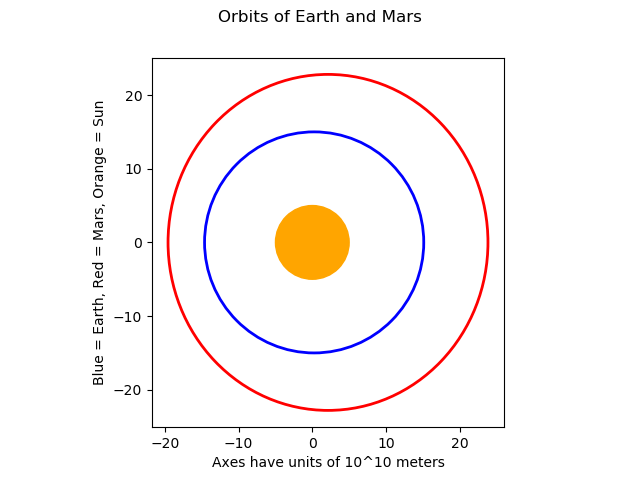
\includegraphics[scale = 0.8]{EllipseTest2.png}
	\label{OrbitPlot}
	\caption{Orbits of Earth and Mars based on Kepler's laws. Orbital tilt is not considered}
\end{figure}

\section{Procedures}
\documentclass{article}
\title{Procedures}
\begin{document}
\section{Equations from Kepler's Laws}
\subsection{Determining Tangential Velocity Given r and Position Given $\theta$}
\label{VelocitySection}
The first step in modeling the orbits of Earth and Mars was to find their tangential velocity at a given radius from
the centre of their elliptical orbit. This was determined using Kepler's law of areas, and one of its resulting 
equations (equations (\ref{Kepler3}) and (\ref{dAandV})), both found in Classical Mechanics by Taylor sections 3.5 and 
8.6, and resulted in equation(\ref{Velocity}) - the equation for L (equation (\ref{L})) was taken from the Georgia State University website in which the eccentricities and semi-major axis values were provided. 
\begin{equation}
	\frac{dA}{dt} = \frac{1}{2}rv_{\theta}
	\label{Kepler3}
\end{equation}
\begin{equation}
	\frac{dA}{dt} = \frac{L}{2\mu}
	\label{dAandV}
\end{equation}
\begin{equation}
	L =\mu\sqrt{GMa(1-e^2)}
	\label{L}
\end{equation}
\begin{equation}
	v_{\theta} = \frac{\sqrt{GMa(1-e^2)}}{r}
	\label{Velocity}
\end{equation}
Equation (\ref{ellipse}) was formed through reference to Classical Mechanics by Taylor secton 8.6. 
Equation (\ref{Radius}) was taken from the Georigia State website. Equation (\ref{difference}) was based on common
knowledge. 
\begin{equation}
	\frac{x^2}{a^2}+\frac{y^2}{b^2} = 1
\end{equation}
\begin{equation}
	\frac{b}{a} = \sqrt{1-e^2}
\end{equation}
\begin{equation}
	\frac{x^2}{a^2}+\frac{y^2}{a^2(1-e^2)} = 1
	\label{ellipse}
\end{equation}
\begin{equation}
	r(\theta) = \frac{a(1-e^2)}{1+ecos(\theta)}
	\label{Radius}
\end{equation}
\begin{equation}
	d = \sqrt{(x_{2} - x_{1})^2-(y_{2}-y_{1})^2}, x = rcos(\theta), y = rsin(\theta)
	\label{difference}
\end{equation}
\subsection{Approximating Position at Time t}
In order to find an exact equation for position at time t, one would have to integrate a variation of Kepler's
third law. This was initially attempted, but then abandoned in favor of an approximation using the equations listed in
section \ref{VelocitySection}. First, functions were defined for equations (\ref{Velocity}) and (\ref{Radius}). Then, a funtion called DeltaT was used to approximate the time elapsed between two tenths of a degree. Next, a distance function was written which takes a inputed time and adds predetermined $\Delta$t's in a while-loop until it reaches the given time. As these chuncks of time are summed, the function also sums the degrees elapse; the sum of the degrees is the actual output of the function. 

The results of the distance funtion and the radius function are then fed into a function which converts the polar coordinates to cartesian coordinates, and then into a function which determines the distance between the planets using equation (\ref{difference}).
\section{}
\end{document}

%\section{Data}
%\documentclass{article}
%\usepackage{graphicx}

%\title{Data Analysis}
%\begin{document}
\section{Initial Results}
Since the distance traveled is calculated in tenths of a degree, the computer used was not powerful enough to plot
a full year in any reasonable amount of time. The best that could be done was a period of ten days. Since the velocity
takes units of meters per second, time was fed in in intervals of 86400 seconds. The resulting graph of the distance
between Earth and Mars, Figure (\ref{DiffPlot}), was unreasonable. Since Earth is closer to the sun, its average radius
will be lower. According to the velocity equation given in the last section, this means the average velocity of Earth 
should be considerably higher than that of Mars. Thus, Earth should make a full orbit before returning to close
proximity with Mars. This should put the time period of the Earth-Mars distance on the scale of about a year.
However, figure (\ref{DiffPlot}) shows an orbital period of about 15 Days. This could have been due to Earth's speed 
being calculated too high but figure(2) shows that both planets take a maximum velocity at their 
semimajor axis, and a minumum 180 degrees after. This is to be expected from equations of the form $a(1+cos(\theta))$ where a is a constant. 
%I realize that typing Figure(2) is unprofessional but no matter how many times I typed the reference it still put 
%figure(1) for some odd reason
\begin{figure}
	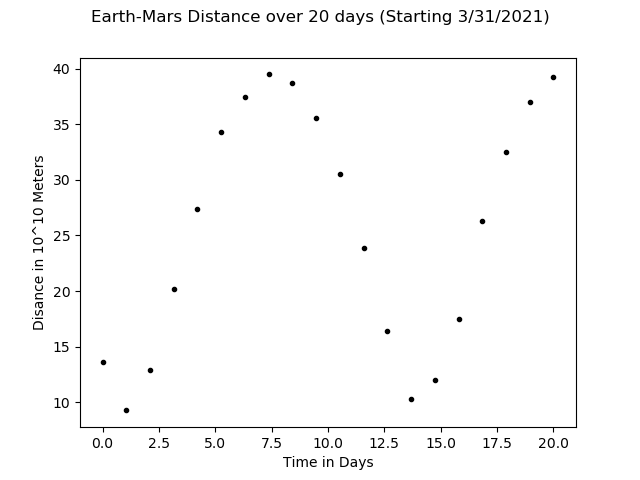
\includegraphics[scale = 0.8]{DistancePlot.png}
	\label{DiffPlot}
	\caption{Distance between Earth and Mars over time as determined by the equations from Section 1.1.1}
\end{figure}

\begin{figure}
	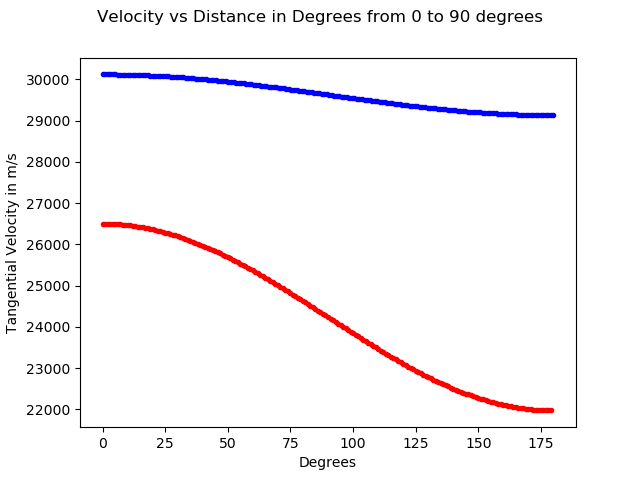
\includegraphics[scale = 0.8]{VelocityPlot.png}
	\label{VelocityPlt}
	\caption{Velocity of Earth and Mars over 180 degrees of rotation}
\end{figure}

\section{Trouble Shooting}
The issue appeared to be the width of the $\Delta\theta$ intervals, as a larger interval will result in a decreasingly
accurate velocity - this is expanded on in section \ref{VelErrSec}. To test this, another plot was generated with $\Delta\theta$ = 1 degree rather than 1 tenth of a degree. Were this the cause for the smaller distance period, the new
figure would have a noticably smaller orbital period. However, the new plot (figure (\ref{DiffPlot2})), while less 
accurate, has roughly the same distance period. All of the constants used in the program were double and triple 
checked, but the source of this strangely small distance period is still unclear.
\begin{figure}
	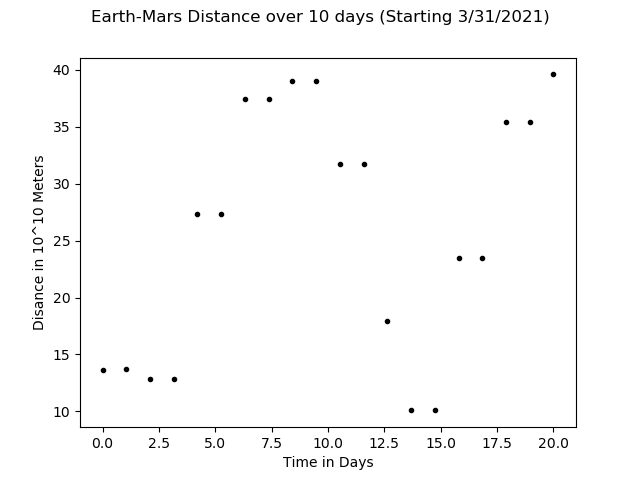
\includegraphics[scale = 0.8]{DistancePlot2.png}
	\label{DiffPlot2}
	\caption{Plot of Difference over time where the $\Delta\theta$ = 1 degree}
\end{figure}
\section{Visualizing Velocity Error}
\label{VelErrSec}
It is helpful to visualize the error in the approximation of constant velocities over small intervals of $\Delta\theta$.
In order to get an idea of the error of assuming these constant velocities, it is helpful compare the starting velocity
of an interval (the one used) to the velocity half way through that interval. This error is shown in equation \ref{Error},
where $v_{1}$ is the velocity at one tenth of the corresponding value on the x-axis and $v_{2}$ 
is the velocity 0.05 degrees later. Figure(\ref{ErrPlot}) shows that the error peaks out at 90 degrees and never exceeds
.0014\%. While this would seem to indicate that the method is reliable, the final results make this doubtful.
\begin{equation}
	Error = \frac{|v_{2}-v_{1}|}{v_{2}}100
	\label{Error}
\end{equation}
\begin{figure}
	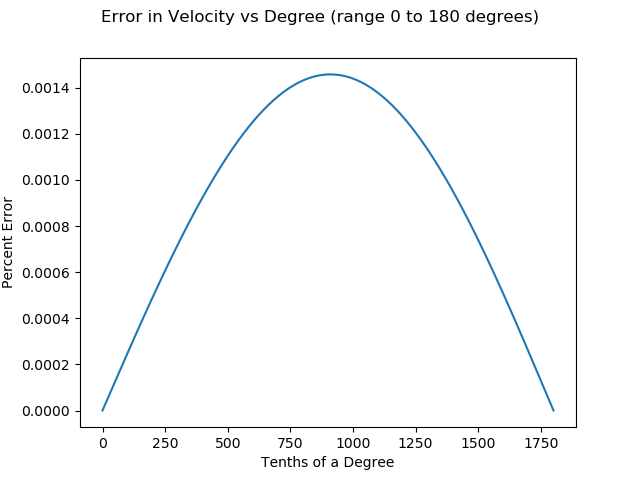
\includegraphics[scale = 0.8]{VelocityError.png}
	\label{ErrPlot}
	\caption{Error based on variation of velocity between two tenths of a degree}
\end{figure}
%\end{document}

\section{Conclusion}
%\documentclass{article}
%\begin{document}
If the only issue with this method of approximation is the width of the $\Delta\theta$ interval, than it should work
fine with a more powerful computer. If, however, it is a more fundamental issue with the method which was somehow
overlooked, more work will need to be done. Based on this project alone, it at least seems that Kepler's laws were
effectivley formatted into equations of velocity capable of being computed quickly and accurately. Formulas that
could integrate the velocity equation directly could be used to better analyze the error of this method.
%\end{document}

\bibliographystyle{plain}
\bibliography{References1}
\end{document}

%\section{Bibliography}
%       \bibitem[Taylor, 2005]{taylor} Taylor, John r., Classical Mechanics. University Science Books, 2005, pg. 93,
        %       309-315.
%       \bibitem[Kepler's Laws, 2016]{georgia1} Hyper Physics. Kepler's Laws. Georgia State University, 2016,http://hyperphysics.phy-astr.gsu.edu/hbase/hph.html. Accessed 31 March, 2021.
%       \bibitem[Developing Kepler's Law of Orbits, 2016]{georgia2} Hyper Physics. Developing Kepler's Law of Orbits. Georgia State University, 2016, http://hyperphysics.phy-astr.gsu.edu/hbase/Mechanics/keplerd.html#c2. Accessed 31 March, 2021.
%        \bibitem[INOVA, 2010]{scope} INOVA. Solar System Scope. INOVA, 2010, https://www.solarsystemscope.com/. Accessed 31 March, 2021.

%\end{thebibliography}
%@book{taylor, 
%	title = {Classical Mechanics},  
%	author = {John r. Taylor}, 
%	year = {2005}, 
%	publisher = {University Science Books}, 
%	pages = {93, 309-315}
%}

%@online{georgia, 
%	author = {Hyper Physics}, 
%	title = {Kepler's Laws}, 
%	year = {2016},
%	url = {http://hyperphysics.phy-astr.gsu.edu/hbase/hph.html}, 
%	urldate = {2021-04-01}
%}

%@online{georgia2, 
%	author = {Hyper Physics}, 
%	title = {Developing Kepler's Law of Orbits}, 
%	year = {2016}, 
%	publisher = {Georgia State University}, 
%	url = {http://hyperphysics.phy-astr.gsu.edu/hbase/Mechanics/keplerd.html#c2}, 
%	urldate = {2021-04-01}
%}

%@online{scope, 
%	title = {Solar System Scope}, 
%	year = {2010}, 
%	url = {https://www.solarsystemscope.com/},
%	publisher = {INOVE}, 
%	urldate = {2021-04-01}
%}
